\section{Results and Scalability of Coordinate Descent}
%\textbf{Coordinate Descent comparison to CLEAN reconstruction}
Show the imaging results on simulated meerkat data.

Show scalability on the numbers of real meerkat observations

Proof-of-concept algorithms was not possible to calculate on real observations. Data too big, reading the data alone is a challenge.



\subsection{Imaging on Simulated Data}
The simulation was created with the Meqtrees Software package, using default settings. The simulations contain [only little gaussian noise on the Visibiliites]. The simulated data is therefore perfectly calibrated, the image reconstruction has to deal with the two fundamental issues of incomplete measurements and non-uniform sampling only.

Free parameter $\lambda$ was fixed on both tests. 4 Full iterations.

CLEAN parameters

Two simulations, one of point sources in figure \ref{results:point} and one of mixed sources in figure \ref{results:mixed}. Two fundamental properties. Two point sources checks the super-resolution capability. Mixture of gaussian and point sources. 

\begin{figure}[h]
	\centering
	\begin{subfigure}[b]{0.45\linewidth}
		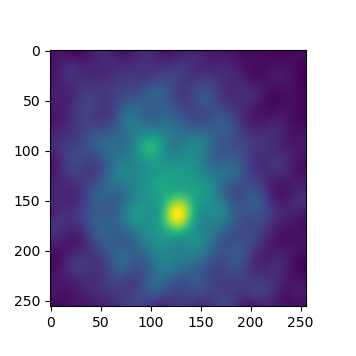
\includegraphics[width=\linewidth]{./chapters/05.algorithms/sim02/sim02_point_dirty.png}
		\caption{Dirty Image of two point sources}
		\label{results:point:dirty}
	\end{subfigure}
	\begin{subfigure}[b]{0.45\linewidth}
		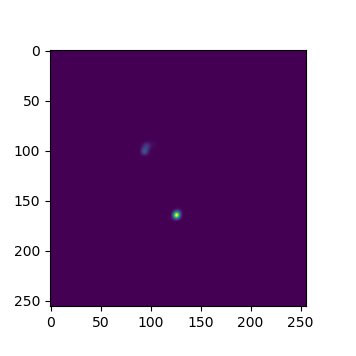
\includegraphics[width=\linewidth]{./chapters/05.algorithms/sim02/image4.png}
		\caption{Reconstruction after 4 Full iterations}
		\label{results:point:cd}
	\end{subfigure}
	\caption{Image reconstruction on two point sources.}
	\label{results:point}
\end{figure}

faint source is spread more widely. Not good, The paper \cite{starck2015starlet} used different $\lambda$ values for different starlet levels. Maybe with this it can be forced to do more precise results, but it was not tried in this work.


Mixed sources, 

\begin{figure}[h]
	\centering
	\begin{subfigure}[b]{0.45\linewidth}
		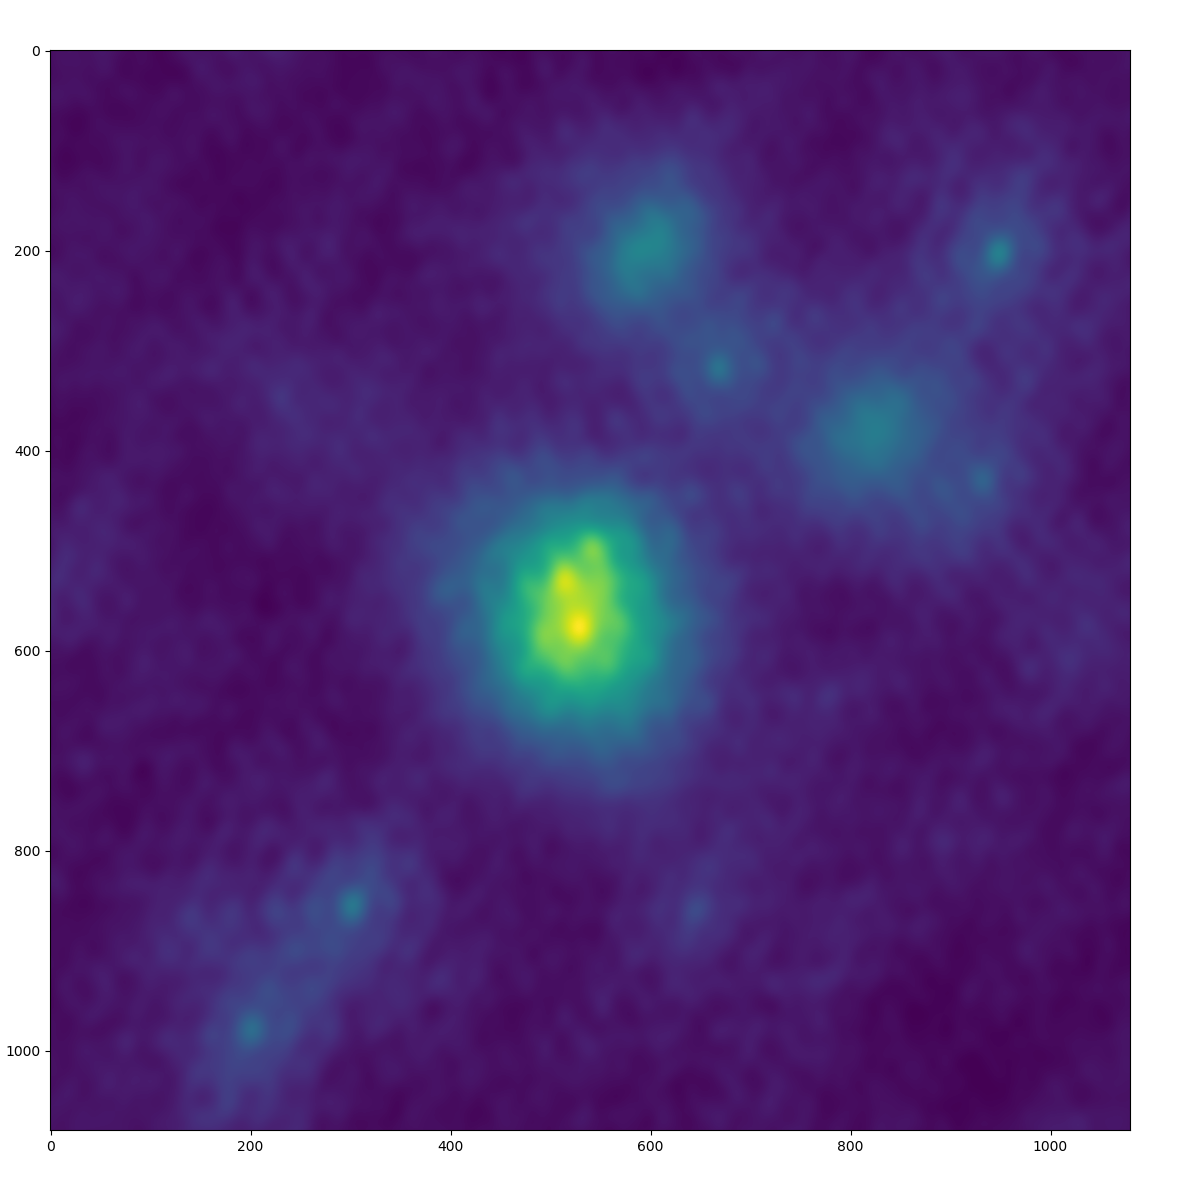
\includegraphics[width=\linewidth]{./chapters/05.algorithms/results/sim00_mixed_sources_dirty.png}
		\caption{dirty image}
		\label{results:g55:nrao:rec}
	\end{subfigure}
	\begin{subfigure}[b]{0.45\linewidth}
		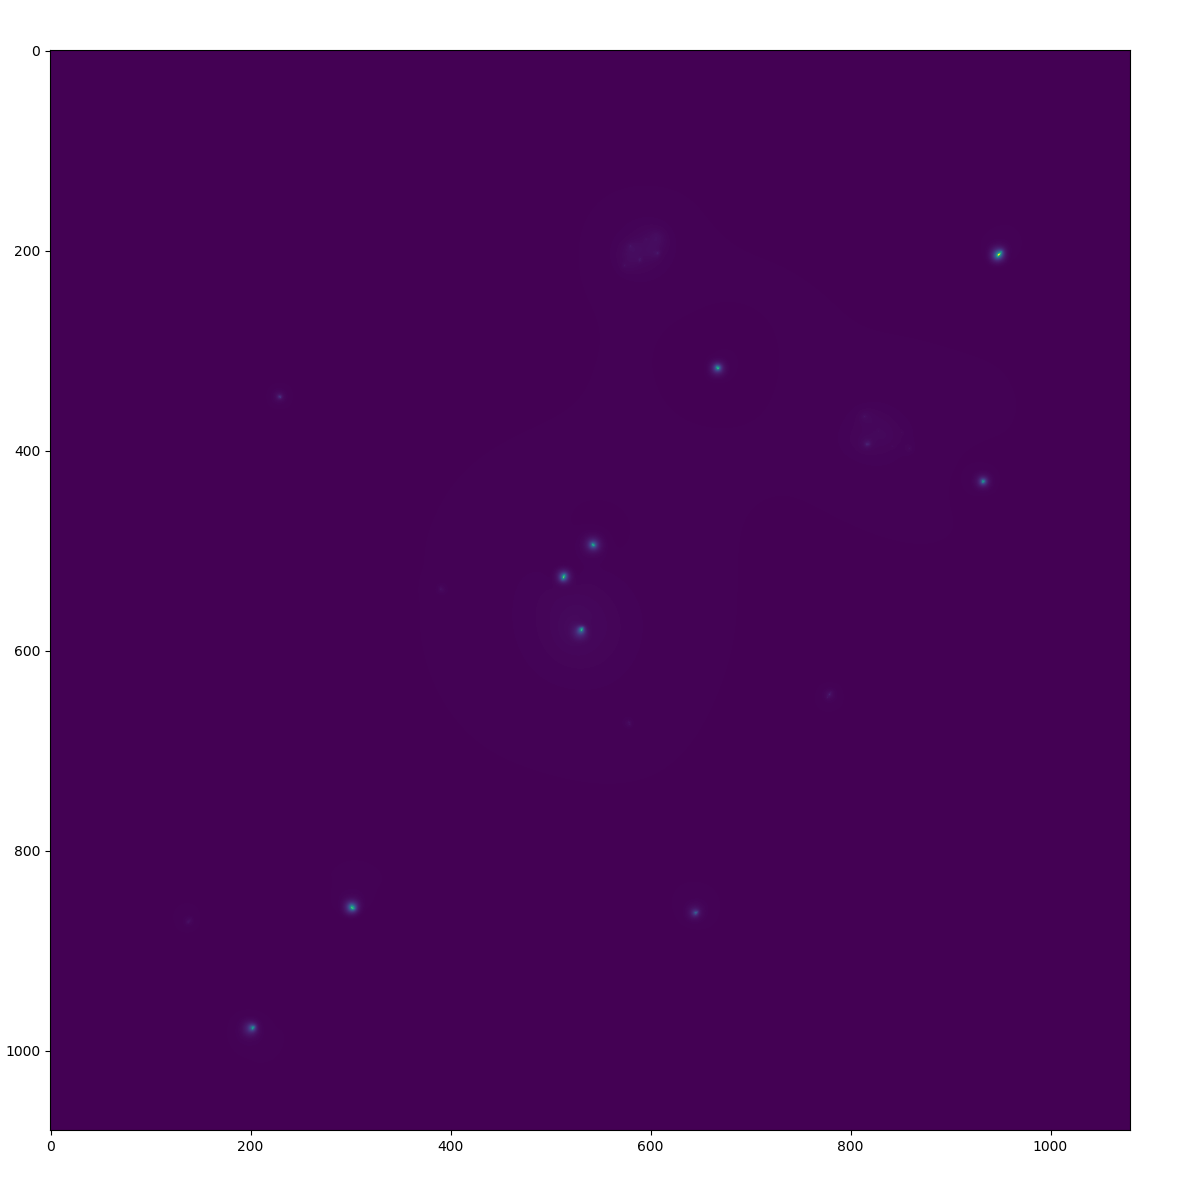
\includegraphics[width=\linewidth]{./chapters/05.algorithms/results/image4.png}
		\caption{Reconstruction after 4 Full iterations}
		\label{results:g55:nrao:dirty}
	\end{subfigure}
	\caption{Reconstruction on mixed sources}
	\label{results:mixed}
\end{figure}

Proper model for extended emissions. CLEAN reconstructs too much flux for the extended emissions.

Not all point sources were detected in the 4 iterations of CD.



\subsection{Scalability of CLEAN and Coordinate Descent}


\begin{figure}[h]
	\centering
	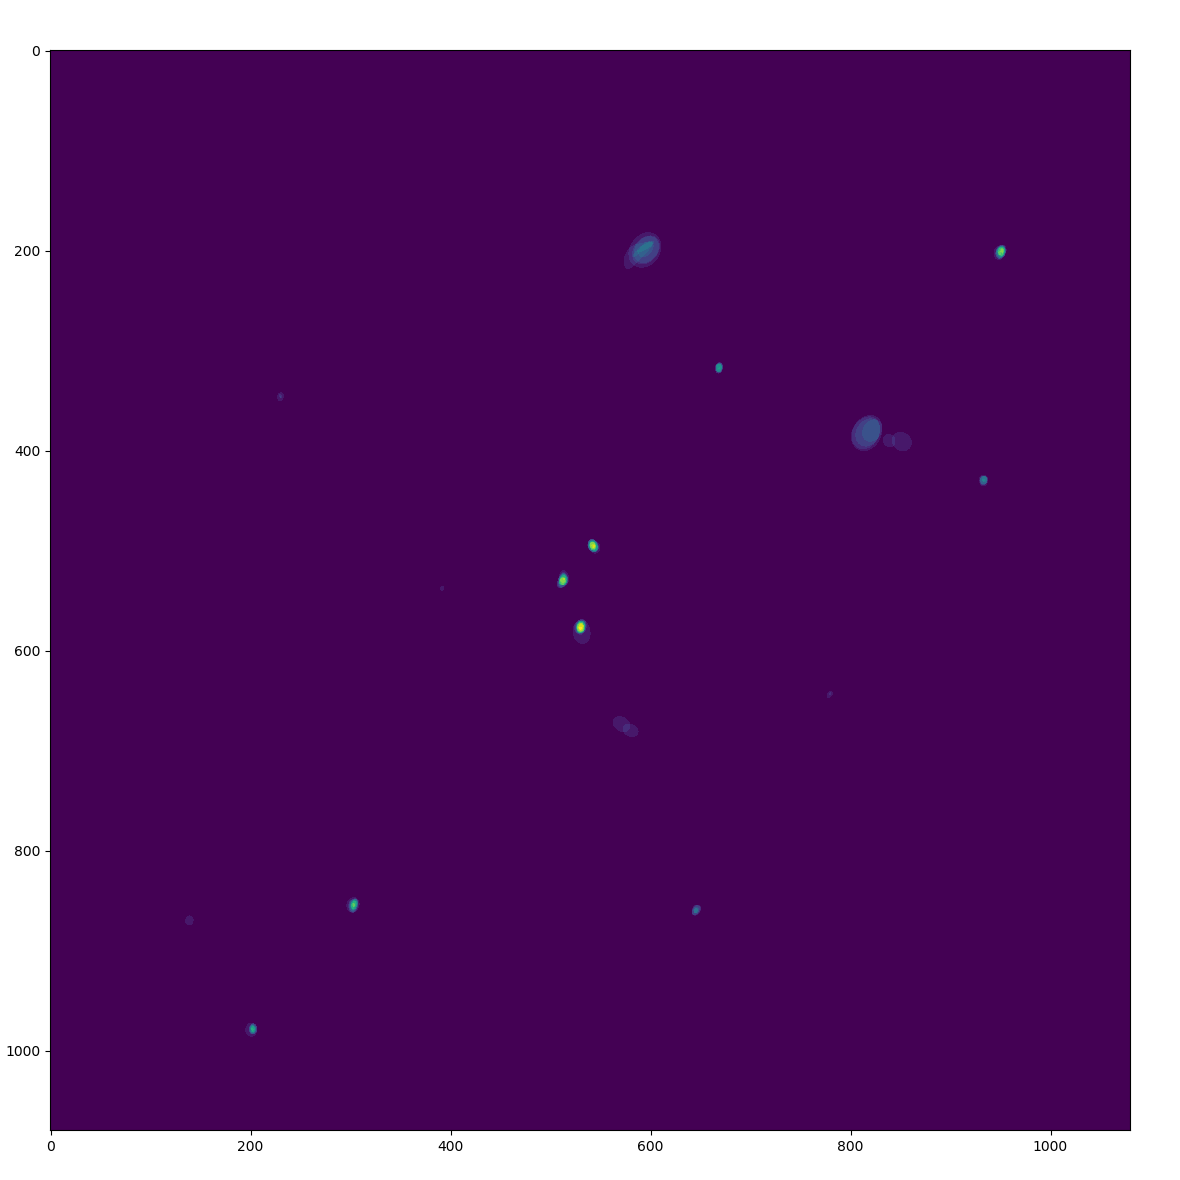
\includegraphics[width=0.5\linewidth]{./chapters/05.algorithms/sim00/full_cache_debug.png}
	\caption{Pixels used to reconstruct the image}
	\label{results:pixels:used}
\end{figure}
Runtime depends heavily on how many columns of the Fourier Transform matrix we need to calculate. Depends on how many starlets are needed to represent a given image, and depends on how well our heuristic captures them. 

Both, CLEAN depends on approximation, which are hard to calculate an "average case complexity". 
Coordinate Descent uses heuristics. Also, average case analysis is difficult. 

Number of Visibilities $M$

Number of Pixels $N$

\subsubsection{Best Case for Coordinate Descent}
Oracle performance of 

Convergence is hard to determine in general. Following simplified assumptions were made: We have a heuristic with oracle performance. It returns only the locations of $\alpha$ in constant time. Furthermore, we assume all axes are independent from each other, only one descent per non-zero axis is necessary.
$S$

\begin{alignat*}{1}
	\text{creating} \:S\: \text{columns of}\: F^{-1} &: S*3M\\
	\text{locating} \:S\: \text{minima of} \:S\: \text{parabolas} &: S*8M\\
	\text{calculating} \:J\: \text{Starlet layers} &: J * 2M
\end{alignat*}


$res * starlet = M$
descent:
$gen fcol = 3*M$
$a = 3 * M$
$b = 4 * M$
$residuals, fcol*diff =  M$

$total_mit_gencol = 11M$

\begin{equation}\label{results:cd:omega}
	\Omega_{CD}(M, S, J) = S*3M + S * 8M + J * 2M
\end{equation}

$S$ depends on the image content directly. For example if the image contains 15 point sources and five Gaussian extended emissions, then $S$ equals 20 non-zero components (if we assume the Gaussian sources require only one starlet for representation). Coordinate Descent therefore is independent of the image size $N$. It solely depends on the size of the measurements $M$, and the number of non-zero components in the dictionary $S$. 

It does not use any approximation for the fourier transform.

Assumptions for $J$ = 10

\subsubsection{CLEAN worst case}

\begin{alignat*}{1}
	\text{non-uniform FFT} &: M + 2N*ld(2N)\\
	\text{non-uniform FFT with} \:w\text{-stacking} &:M + W*(2N*ld(2N) + 2N) + N*ld(N)\\
	D\: \text{CLEAN deconvolution} &: D*2N
\end{alignat*}

(Cite New W-stacking approach)
Nufft: $M + 2N log 2N$
W-stacking = $M + W*(2N log 2N + 2N) + N log N$
Deconvolution = $D*2N$


\begin{equation}
O_{CLEAN}(M_{Major}, M, N,  W, D) = M_{Major} * [M + [W*(2N log 2N + 2N) + N log N] + D*2N]
\end{equation}

Complex formula. But for MeerKAT, the number of Visibilities $M$ is by far the largest. Simplifies to $M_{Major}*M$

Assumptions
Estimates for $M_{Major}$ = 10. (Cite New W-stacking approach)
W = $100$ depends on observation between 10, and hundreds. Depends on the observation. Cite new w-stacking approach can limit the number of w-stacks. 
D=35'000

\subsubsection{Runtime Complexity on real MeerKAT data}
In terms of $S$ for 
Where the data comes from

Calibration: 
Visibilities = 4060770
Channels = 540

pixels = 8192 * 8192 = 67 108 864

Target, what would an Ideal Compressed Sensing implementation do.

Memory requirement

MeerKAT has by far more Visibilities than pixels

Write one meerkat observation

The number of $S$ and then the lower bound of Coordinate Descent. (Put WSCLEAN image in here and Discuss $S$)



Other compressed sensing approaches have a more expensive term than $D*2N$ for their complexity. But compared to compressed sensin.


IMAGE CONTENT SCALES WITH pixels instead of Visibilities.

